\subsection{球的体积}\label{subsec:2-12}
\begin{enhancedline}

和柱体、锥体一样,也可以应用\hyperref[zgyl]{祖暅原理}推出球体的体积公式。

我们先研究半径为 $R$ 的半球。 为了应用\hyperref[zgyl]{祖暅原理},需要找到一个能够求体积的几何体,
使它和半球可夹在两个平行平面之间,当用平行于这两个平面的任意一个平面去截它们时,截得的截面面积总相等。

为此,我们取一个底面半径和高都等于 $R$ 的圆柱,从圆柱中挖去一个以圆柱的上底面为底面,
下底面圆心为顶点的圆锥,把所得的几何体和半球放在同一个平面 $\alpha$ 上(图 \ref{fig:ltjh-2-72})。
因为圆柱的高等于 $R$,所以这个几何体和半球都夹在两个平行平面之间。

\begin{figure}[htbp]
    \centering
    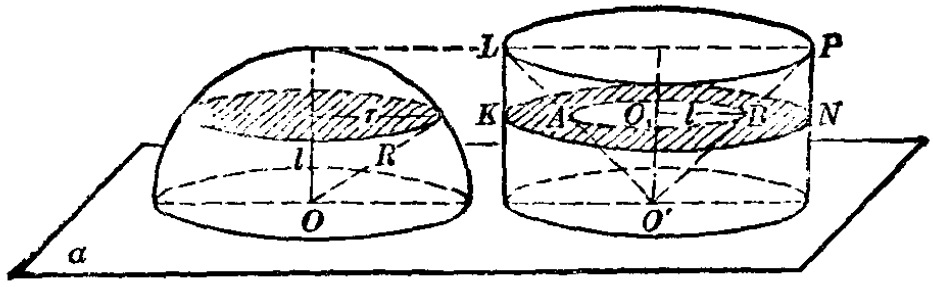
\includegraphics[width=13cm]{../pic/ltjh-ch2-72.png}
    \caption{}\label{fig:ltjh-2-72}
\end{figure}

用平行于平面 $\alpha$ 的任意一个平面去截这两个几何体,截面分别是圆面和圆环面。
如果截平面与平面 $\alpha$ 的距离为 $l$,那么圆面半径 $r = \sqrt{R^2 - l^2}$,
圆环面的大圆半径为 $R$,小圆半径为 $l$(因为 $\triangle O'O_1B$ 是等腰三角形)。因此
\begin{gather*}
    S_\text{圆} = \pi r^2 = \pi (R^2 - l^2) \douhao \\
    S_\text{圆环} = \pi R^2  - \pi l^2 = \pi (R^2 - l^2) \douhao
\end{gather*}

$\therefore$ \quad $S_\text{圆} = S_\text{圆环}$。

根据\hyperref[zgyl]{祖暅原理},这两个几何体的体积相等,即
$$ \exdfrac{1}{2} V_{\text{球}} = \pi R^2 \cdot R - \exdfrac{1}{3} \pi R^2 \cdot R  = \exdfrac{2}{3} \pi R^3 \juhao $$

所以 \qquad $V_{\text{球}} = \exdfrac{4}{3} \pi R^3$。

由此,我们得到下面定理:

\begin{dingli}[定理][dl:qiu-tj]
    如果球的半径是 $\bm{R}$,那么它的体积是
    \begin{center}
        \framebox[10em]{$\bm{V_\text{球} = \exdfrac{4}{3} \pi R^3}$。}
    \end{center}
\end{dingli}

\liti[0] 有一种空心钢球,重 142 g,测得外径等于 5.0 cm。 求它的内径(钢比重是 $7.9\;\kmlflm$)。

\jie 设空心钢球的内径为 $2x$ cm,那么钢球的重量是
\begin{gather*}
    7.9 \cdot \left[ \exdfrac{4}{3} \pi \cdot \left( \exdfrac{5}{2} \right)^3 - \exdfrac{4}{3} \pi x^3 \right] = 142 \douhao \\
    x^3 = \left( \exdfrac{5}{2} \right)^3 - \dfrac{142 \times 3}{7.9 \times 4 \pi} \approx 11.3 \juhao
\end{gather*}

$\therefore$ \quad $x \approx 2.24$,

\qquad $2x \approx 4.5\;(\limi)$。

答:空心钢球的内径约为 4.5 厘米。


\begin{lianxi}

\xiaoti{球面面积膨胀为原来的二倍,计算体积变为原来的几倍。}

\xiaoti{一个正方体的顶点都在球面上,它的棱长是 4 cm,求这个球的体积。}

\end{lianxi}

\end{enhancedline}

